\documentclass{standalone}
\usepackage{tikz, ifthen}
\usepackage{amsmath}

\begin{document}

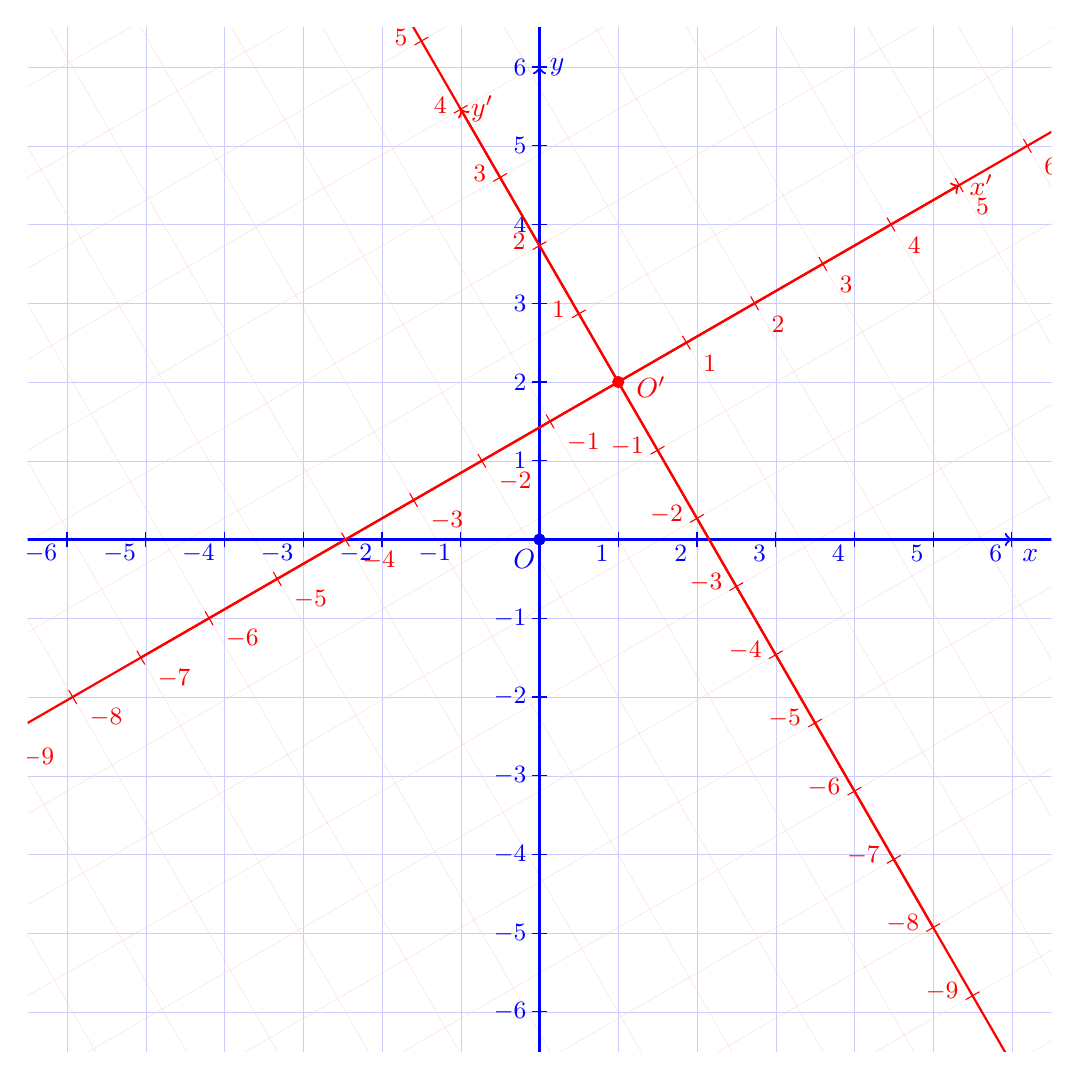
\begin{tikzpicture}
    
    % Center of the circle
    \def\xmin{-6}
    \def\xmax{6}
    \def\ymin{-6}
    \def\ymax{6}
    \def\dx{.5}
    \def\dy{.5}
    \def\xminb{\xmin-\dx}
    \def\xmaxb{\xmax+\dx}
    \def\yminb{\ymin-\dy}
    \def\ymaxb{\ymax+\dy}
    \def\xo{1}    % translation, x
    \def\yo{2}    % translation, y
    \coordinate (oo) at (\xo, \yo);
    \def\xpmin{-6}
    \def\xpmax{ 6}
    \def\ypmin{-5.5}
    \def\ypmax{ 5.5}
%   \def\a{0.5};
%   \coordinate (fa) at (\xa, \ya);
%   \coordinate (fb) at (\xb, \yb);
%   \def\c{sqrt((\xa-\xb)^2+(\ya-\yb)^2)/2};
%   \def\xc{0.5*(\xa+\xb)};
%   \def\yc{0.5*(\ya+\yb)};
%   \coordinate (center) at ({\xc}, {\yc});
%   \def\b{sqrt(\c^2-\a^2)};
%   \def\alpha{{atan2(\yb-\ya,\xb-\xa)}};

    \clip (\xminb, \yminb) rectangle (\xmaxb, \ymaxb);
    % Fill outside region
    \begin{scope}
        % \fill[gray!30] (\xmin, \ymin) rectangle (5, \ymax);
        % \fill[gray!30] (center) circle (3);
    \end{scope}

%   % Hyperbola
%   \draw[thick, black, fill=white] plot[parametric, domain=-2.8:2.8] 
%       ({\xc+\a*cosh(\x)}, {\yc+\b*sinh(\x)}); % Draw the parametric line

    % Draw grid
    \draw[step=1., blue!20, ultra thin] (\xmin-2, \ymin-2) grid (\xmax+2, \ymax+2); % Visible grid with lighter color
%   % Draw grid
    \draw[step=1., red!20, ultra thin, rotate around={30:(oo)}] (\xmin-4,\ymin-4) grid (\xmax+4, \ymax+4); % Visible grid with lighter color
    % Axes, x
    \draw[->, thick, blue] (\xmin, 0) -- (\xmax, 0) node[below right] {$x$};
    \draw[    thick, blue] (\xmin-2, 0) -- (\xmax+2, 0);
    \draw[->, thick, blue] (0, \ymin) -- (0, \ymax) node[right] {$y$};
    \draw[    thick, blue] (0, \ymin-2) -- (0, \ymax+2);
    % Axis ticks
    \foreach \x in {\xmin,..., \xmax}{
        \ifthenelse{ \x = 0 }{}{\draw[blue] (\x, -0.1) -- (\x, +0.1) node[below=8pt, left=0pt] {\small $\x$};}
    }
    \foreach \y in {\ymin,..., \ymax}{
        \ifthenelse{ \y = 0 }{}{\draw[blue] (-0.1, \y) -- (0.1, \y) node[left=4pt] {\small $\y$};}
    }

    % Axes, x'
    \draw[->, thick, red, rotate around={30:(oo)}] (\xmin, \yo) -- (\xmax, \yo) node[right] {$x'$};
    \draw[->, thick, red, rotate around={30:(oo)}] (\xo, \ymin) -- (\xo, \ymax) node[right] {$y'$};
    \draw[    thick, red, rotate around={30:(oo)}] (\xmin-2, \yo) -- (\xmax+2, \yo);
    \draw[    thick, red, rotate around={30:(oo)}] (\xo, \ymin-2) -- (\xo, \ymax+2);
    % Axis thick
    \foreach \x in {-9,..., \xmax}{
        \ifthenelse{ \x = 0 }{}{\draw[red, rotate around={30:(oo)}] (\x+\xo, \yo-0.1) -- (\x+\xo, \yo+0.1) node[below=10pt, right=4pt] {\small $\x$};}
    }
    \foreach \y in {-9,...,\ymax}{
        \ifthenelse{ \y = 0 }{}{\draw[red, rotate around={30:(oo)}] (\xo-0.1, \yo+\y) -- (\xo+0.1, \yo+\y) node[left=4pt] {\small $\y$};}
    }
    % Origin
    \filldraw[blue] (0,0) circle (2pt) node[below=7pt, right=-13pt] {$O$};
    \filldraw[red] (\xo,\yo) circle (2pt) node[below=2pt, right=3pt] {$O'$};

%   \filldraw[blue]  (3,5) circle (1pt) node[below right] {$\equiv (3,5)$};
%   \filldraw[red]   (3,5) circle (1pt) node[below=20pt, right] {$\equiv (1,3.5)$};
%   \filldraw[black] (3,5) circle (2pt) node[below left] {$A$};

%   \filldraw[blue]  (-4,3) circle (1pt) node[below right] {$\equiv (-4,3)$};
%   \filldraw[red]   (-4,3) circle (1pt) node[below=20pt, right] {$\equiv (-6,1.5)$};
%   \filldraw[black] (-4,3) circle (2pt) node[below left] {$B$};

%   \filldraw[blue]  (1,-4) circle (1pt) node[right=12pt] {$\equiv (1,-4)$};
%   \filldraw[red]   (1,-4) circle (1pt) node[right=55pt] {$\equiv (-1,-5.5)$};
%   \filldraw[black] (1,-4) circle (2pt) node[right] {$C$};

%   % Foci
%   \filldraw[blue] (\xa, \ya) circle (2pt) node[above right] {$0$};
%   \filldraw[blue] (\xb, \yb) circle (2pt) node[above right] {$2$};
    
\end{tikzpicture}

\end{document}
